\subsection{Project Requirements} \label{label:projectRequirements}
Number of functional and non-functional requirements have been identified and classified using MoSCoW system during the design stage. 

\subsubsection{Functional Requirements}
Majority of functional requirements have been created based on solver requirements for International Competition on Computational Models of Argumentation 2017. Furthermore, those requirements can be characterized based on their functionality:
\begin{itemize}
	\item Computational functionality - those include all different types of semantics and individual tasks related to them. For example, a requirement will exist for the solver to compute the stable extensions of the given argumentation framework. However, this could be further split up into separate tasks: compute all extensions, some extensions, evaluate if the given argument is skeptically or credulously accepted.
	\item Solver functionality - those include additional requirements that the solver should have. They might include requirements like solver should be able to read \textit{tgf} file and parse the argumentation framework from them, etc.
\end{itemize}

In terms of the computational functionality, Alias is required to solve all semantics identified in section \ref{sec:argumentationSemantics}, which are as follow: complete, stable, preferred and grounded extensions \citep{dung1995}, stage \citep{verheij1996two}, ideal \citep{dung2007computing}, and semi-stable \citep{caminada2006semi} semantics. Although seven individual semantics have been identified as the requirements for the solver, only three of them: complete, stable and preferred, have been classified as \textit{Mush Have} in terms of MoSCoW approach. The proposed semantics are part of the original group of extensions introduced by \citet{dung1995} in his paper. 

Furthermore, as mentioned above, there are number of tasks that the solver should be able to perform for each semantic and as seen in the section \ref{approaches}, those are as follow:
\begin{enumerate}
	\item Given an abstract argumentation framework compute some of the extensions
	\item Given an abstract argumentation framework compute all extensions
	\item Given an abstract argumentation framework and some argument, decide whether the given argument is credulously accepted
	\item Given an abstract argumentation framework and some argument, decide whether the given argument is skeptically accepted
\end{enumerate}

Above tasks are relevant to all semantics with exception to grounded and ideal extensions, where only tasks 1 and 3 can be performed. Hence, it brings up the overall number of tasks for all semantics to 24 separate tasks. Thus, to deliver solution with the most value, for the extensions categorized as \textit{Must Have}, only tasks to compute all extensions have been categorized as \textit{Must Haves}. The remaining tasks for each of them have been classified as \textit{Should Have}. Furthermore, computing all Semi-Stable and Stage extensions have been categorized as \textit{Could Have}, with all the remaining tasks and extensions as \textit{Won't Have}. This can be seen in table \ref{table:moscowSemanticRequirements} and further in the appendix \ref{appendix:requirementAnalysis}. 


% Please add the following required packages to your document preamble:
% \usepackage{multirow}
\begin{table}[]
	\centering
	\caption{MoSCoW qualifications of semantic based requirements}
	\label{table:moscowSemanticRequirements}
	\begin{tabular}{|l|l|l|}
		\hline
		\textbf{Semantic}            & \textbf{Task}                                   & \textbf{MoSCoW} \\ \hline \hline
		\multirow{4}{*}{Complete}    & Compute all extensions                           & Must Have       \\ \cline{2-3} 
		& Compute some extensions                          & Should Have     \\ \cline{2-3} 
		& Decide if argument is credulously accepted & Should Have     \\ \cline{2-3} 
		& Decide if argument is skeptically accepted & Should Have     \\ \hline
		\multirow{4}{*}{Preferred}   & Compute all extensions                           & Must Have       \\ \cline{2-3} 
		& Compute some extensions                          & Should Have     \\ \cline{2-3} 
		& Decide if argument is credulously accepted & Should Have     \\ \cline{2-3} 
		& Decide if argument is skeptically accepted & Should Have     \\ \hline
		\multirow{4}{*}{Stable}      & Compute all extensions                           & Must Have       \\ \cline{2-3} 
		& Compute some extensions                          & Should Have     \\ \cline{2-3} 
		& Decide if argument is credulously accepted & Should Have     \\ \cline{2-3} 
		& Decide if argument is skeptically accepted & Should Have     \\ \hline
		\multirow{4}{*}{Semi-Stable} & Compute all extensions                           & Could Have      \\ \cline{2-3} 
		& Compute some extensions                          & Won't Have      \\ \cline{2-3} 
		& Decide if argument is credulously accepted & Won't Have      \\ \cline{2-3} 
		& Decide if argument is skeptically accepted & Won't Have      \\ \hline
		\multirow{4}{*}{Stage}       & Compute all extensions                           & Could Have      \\ \cline{2-3} 
		& Compute some extensions                          & Won't Have      \\ \cline{2-3} 
		& Decide if argument is credulously accepted & Won't Have      \\ \cline{2-3} 
		& Decide if argument is skeptically accepted & Won't Have      \\ \hline
		\multirow{2}{*}{Grounded}    & Compute all extensions                           & Won't Have      \\ \cline{2-3} 
		& Decide if argument is credulously accepted & Won't Have      \\ \hline
		\multirow{2}{*}{Ideal}       & Compute all extensions                           & Won't Have      \\ \cline{2-3} 
		& Decide if argument is credulously accepted & Won't Have      \\ \hline
	\end{tabular}
\end{table}


The above classification is only concerned with the argumentation semantics and its tasks. Other requirements have been identified that although are not concerned with solving the abstract argumentation semantics are needed for the solver and can improve the system. As an example, Alias should be able to read parse the argumentation framework from the provided file, like \textit{tgf} or \textit{apx}, or from dot graph or even the database. Furthermore, the user should be able to save created argumentation framework in different formats for future use. 

Although original implementation of Alias provides a certain aspects of those requirements, during the development of the new version, the architecture of the system and its implementation will have to be reviewed and modified to allow for the changes.

\subsubsection{Non-Functional Requirements}
Apart from all functional requirements, number of non-functional requirements have also been identified. Those are mostly concerned with the performance and scalability of the proposed solution. Although those do not bring any tangible value to the finished system, those requirements are critical to produce the high performance and scalable system that could match existing solvers in terms of computation time. 

In terms of performance and scalability, the requirement for the Alias is to be able to cope with argumentation frameworks of any size. User should be confident that the application will be able to provide the correct results all time, no matter the size of provided framework. Although, it is difficult to convert it into tangible requirements, the attempt has been made to specify brackets for different sizes of argumentation frameworks: 

\begin{enumerate}
	\item Small - up to 20 arguments and relations
	\item Medium - from 20 up to 100 arguments and relations
	\item Large - above 100 arguments 
\end{enumerate}

However, the above classification is only concerned with the size of graph generated from the argumentation framework. Although this can usually correspond to the complexity of the framework, it is not always the case. For example, argumentation framework shown in figure \ref{fig:mediumAF} consist of only 41 arguments and 73 attacks. However, the testing of proposed solutions showed that although the argumentation framework is of medium size, the complexity of relations between the arguments proved to be challenging due to many arguments defending themselves. Thus, the above classification will only be used for establishing basic requirements for the application to be able to handle all types of argumentation frameworks. 

\begin{figure}[h]
	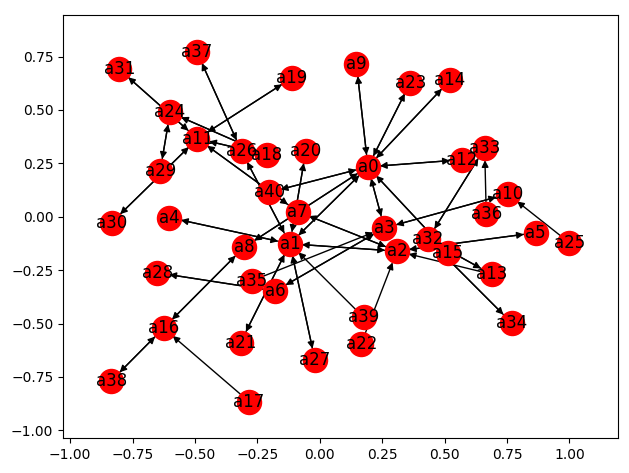
\includegraphics[width=\textwidth]{medium}
	\caption{Medium sized argumentation framework}
	\label{fig:mediumAF}
\end{figure}

Another aspect of non-functional requirements is the ease of use of the application. Original Alias application has been implemented in Python, an interpreted, high-level programming language \citep{millman2011python}. Although Python has been designed as the general purpose language, it became very popular. And with the libraries like NumPy and SciPy, it became a popular choice for high-level scientific code development \citep{perez2011python}. Thus, the Python implementation of abstract argumentation semantics solver without the need to setup the environment in any way prior to using it would be beneficial. Being able to install the Alias from the PyPi, the Python package manager \citep{pypi}, and use it 'out of the box', gives it an advantage over other solvers.
